% Part 1 report: cross-lingual leakage of EMBER, SNMF and SNMF+EMBER on Gemma-2-2B-it.
% Generated from Part1_report.md. Compile from this folder:
%   pdflatex Part1_report && bibtex Part1_report && pdflatex Part1_report && pdflatex Part1_report
% It uses ../acl.sty, ../acl_natbib.bst and ../references.bib. If your setup does not accept the relative
% paths, copy those three files next to this file and remove the "../" below.
\documentclass[11pt]{article}

\usepackage[final]{../acl}

\usepackage{times}
\usepackage{latexsym}
\usepackage[T2A,T1]{fontenc}
\usepackage[utf8]{inputenc}
\usepackage{microtype}
\usepackage{inconsolata}
\usepackage{graphicx}
\usepackage{booktabs}
\usepackage{amsmath}
\usepackage{amssymb}
\usepackage{xcolor}

\graphicspath{{figures/}}

\newcommand{\qatrain}{\textsc{QA}\textsubscript{train}}
\newcommand{\qatest}{\textsc{QA}\textsubscript{test}}
\newcommand{\simdomtrain}{\textsc{SimdomQA}\textsubscript{train}}
\newcommand{\simdomtest}{\textsc{SimdomQA}\textsubscript{test}}
\newcommand{\cyr}[1]{{\fontencoding{T2A}\fontfamily{cmr}\selectfont #1}}

\title{English Edits, Other Languages:\\
Does Concept Erasure Transfer Across Languages?}

\author{Mary Arav \\
  Tel Aviv University \\
  \texttt{maryarav@mail.tau.ac.il} \\\And
  Ori Petel \\
  Tel Aviv University \\
  \texttt{oripetel@mail.tau.ac.il} \\\And
  Semyon Guretskiy \\
  Tel Aviv University \\
  \texttt{semyong@mail.tau.ac.il} \\}

\begin{document}
\maketitle

\begin{abstract}
Concept erasure removes knowledge of a target concept (e.g. \emph{Harry Potter}) from a language model's weights while keeping the rest of the model intact. EMBER, a recent method, does this by editing the input embeddings of a few dozen English tokens. Because those tokens are English, it is unclear whether the erasure still holds when the same concept is asked about in another language. We reproduce three erasure methods from the EMBER paper on Gemma-2-2B-it for all 18 of its concepts: EMBER (an embedding edit), SNMF (an MLP edit) and their combination SNMF+EMBER. We tune every edit in English only and then ask held-out multiple-choice questions in English, German, Spanish, French and Russian. We measure \emph{retention} (how much of the concept survives, relative to the unedited model in the same language) and \emph{leak} (retention in a language minus retention in English).

EMBER leaks: its mean leak is +0.19 (95\% CI [+0.11, +0.27]), and in Russian it is +0.33, with Russian retention at 0.96, almost as if nothing had been erased. SNMF does not leak (+0.01, [$-$0.07, +0.08]), but it removes 24--41\% of similar-domain knowledge and lowers English MMLU from 0.553 to 0.506. SNMF+EMBER erases English the most (retention 0.39). It does not leak into German, Spanish or French, but it still leaks into Russian (+0.23, [+0.08, +0.38]). Along the way we found that the original multiple-choice scorer cut answers off after four tokens, which counted correct answers as ``erased'' and inflated the erasure of the embedding-based methods. We fixed the scorer, re-selected all edits and re-ran every evaluation.
\end{abstract}

\section{Introduction}\label{sec:1}

A model may need to forget a concept for safety, copyright or privacy reasons. Persistent concept erasure changes the model's weights so that it can no longer use knowledge about the concept, while its other knowledge and its ability to write fluent text stay intact. A known weakness of current methods is that the erasure is shallow: the knowledge can come back after a little fine-tuning, a rephrased question, or a different question format \citep{deeb2024unlearning,lynch2024eight,hong2025intrinsic,ye2025formindependent}.

\citet{suslik2026ember} argue that part of the problem is that most erasure methods edit only the MLP layers and ignore the embedding layer, where token-level knowledge is also stored. Their method, EMBER, finds concept features in the embedding matrix and subtracts them from the embeddings of a small set of concept tokens. Added to MLP-based methods, it improves erasure and makes it much more robust to relearning.

EMBER's features and edited tokens all come from English Wikipedia text. An embedding edit changes specific rows of the vocabulary, and a question in another language, particularly one written in another script, may never touch an edited row. The EMBER paper names this as a limitation (``Language coverage''), but it does not measure it. We therefore ask: \emph{if an erasure is tuned in English, does the concept re-emerge when the same questions are asked in another language, and does this differ between embedding-based and MLP-based erasure?}

To answer this, we reproduce three methods from the EMBER paper (EMBER, SNMF and SNMF+EMBER) on Gemma-2-2B-it for all 18 of its concepts. We replace the paper's paid Gemini judge with a local judge and validate it against Gemini, and we select one edit per concept and method using English data only. We then translate the evaluation questions into German, Spanish, French and Russian, apply each English edit once without re-tuning, and measure how much of the concept survives in each language. In the course of this work we also found and corrected an answer-parsing problem in the original multiple-choice scorer (Section~\ref{sec:3.5}).

Our main findings are as follows.

\begin{itemize}
\setlength\itemsep{1pt}
\item EMBER leaks: the concept survives better in every other language than in English, and almost fully in Russian.
\item SNMF erases about evenly across languages, but it damages related and general knowledge more.
\item SNMF+EMBER erases English the most and leaks only into Russian, the one tested language with a different script.
\item With the original scorer our numbers match those of the EMBER paper closely, but that scorer overstates the erasure of the embedding-based methods.
\end{itemize}

\section{Background}\label{sec:2}

\subsection{Concept erasure}\label{sec:2.1}

Given a model $M$ and a concept $C$, the goal is an edited model $M'$ that answers questions about $C$ at chance level while keeping its performance on everything else. Methods differ in where they intervene. Fine-tuning methods such as RMU \citep{li2024wmdp} and CRISP \citep{ashuach2026crisp} train the model with a forgetting objective. Localize-then-edit methods such as PISCES \citep{gurarieh2025precise}, SNMF \citep{shafran2026constructing} and EMBER \citep{suslik2026ember} first find concept-related features and then remove them directly from the weights, without training.

\subsection{EMBER: erasing from the embedding matrix}\label{sec:2.2}

EMBER works in three steps. First, it takes the tokens that appear in 300 concept sentences ($\mathcal{S}_C$) and 300 neutral Wikipedia sentences ($\mathcal{S}_N$) and factorizes their embeddings with a sparse matrix factorization, $E^{\top}\approx ZY$, keeping only the top 1\% of coefficients per feature. Each column of $Z$ is then a direction shared by a small group of tokens. Second, it keeps the features whose coefficient mass is at least $\tau=2$ times larger on concept-only tokens than on neutral tokens, and an LLM confirms that the feature's tokens are about the concept. Third, for each concept token $t$ that uses a concept feature, it subtracts that feature's contribution:

\begin{equation*}
\mathbf{e}_t \leftarrow \mathbf{e}_t - \delta \sum_{i \in \mathcal{F}_C} Y_{i,t}\,\mathbf{z}_i,
\end{equation*}

where $\delta$ is the erasure strength: $\delta = 1$ removes exactly the recovered component and $\delta > 1$ over-subtracts.

On Gemma this edits only 31--86 tokens per concept (31--86, mean 57, in our runs, the same range as in the paper); the remaining vocabulary of 256,000 tokens is untouched. As a consequence, a question that expresses the concept with other tokens, for example the Russian \emph{\cyr{Хогвартс}} instead of \emph{Hogwarts}, reads embeddings that were never edited.

\subsection{SNMF: erasing from the MLP layers}\label{sec:2.3}

SNMF applies a semi-nonnegative matrix factorization to the MLP activations on $\mathcal{S}_C\cup\mathcal{S}_N$, layer by layer. It selects concept features in the same way (ratio test followed by an LLM check) and removes each feature direction $\mathbf{f}$ from the MLP weights by directional ablation \citep{arditi2024refusal}, $W\leftarrow W-\delta\,\mathbf{f}\mathbf{f}^{\top}W$. This is done separately for the input weights (strength $\delta_{\mathrm{in}}$, a chosen range of layers) and the output weights (strength $\delta_{\mathrm{out}}$, another range of layers). Since the edit lies inside the network, it does not depend on which input tokens a question uses.

\subsection{SNMF+EMBER}\label{sec:2.4}

SNMF+EMBER is the main configuration of the EMBER paper. The concept's EMBER edit, with its selected $\delta$, is applied first, and the SNMF grid is then searched again on top of it.

\subsection{Cross-lingual knowledge}\label{sec:2.5}

Multilingual models share much of their factual knowledge across languages in their middle layers \citep{wendler2024llamas}. Safety behaviour trained in English, however, often fails in other languages \citep{deng2024multilingual,yong2023lowresource}, and knowledge edits made in English transfer mainly to languages close to English \citep{qi2023crosslingual,wang2024crosslingualediting}. An embedding edit is a special case: it is tied to specific vocabulary rows, so it cannot directly change a word that is spelled with other tokens.

\section{Experimental setup}\label{sec:3}

Figure~\ref{fig:1} gives an overview of the experiment. For each concept and method we search a grid of erasure configurations, for example how strongly to erase and in which layers, and score every configuration with a single number that rewards forgetting the concept while keeping everything else intact. This search uses English data only. The selected configuration is then applied once to the model, again without any language-specific tuning, and the edited model is evaluated on how well it forgets the concept in English and in four other languages. The question is whether the concept can still be accessed in other languages and how strong the leakage is.

\begin{figure*}[t]
\centering
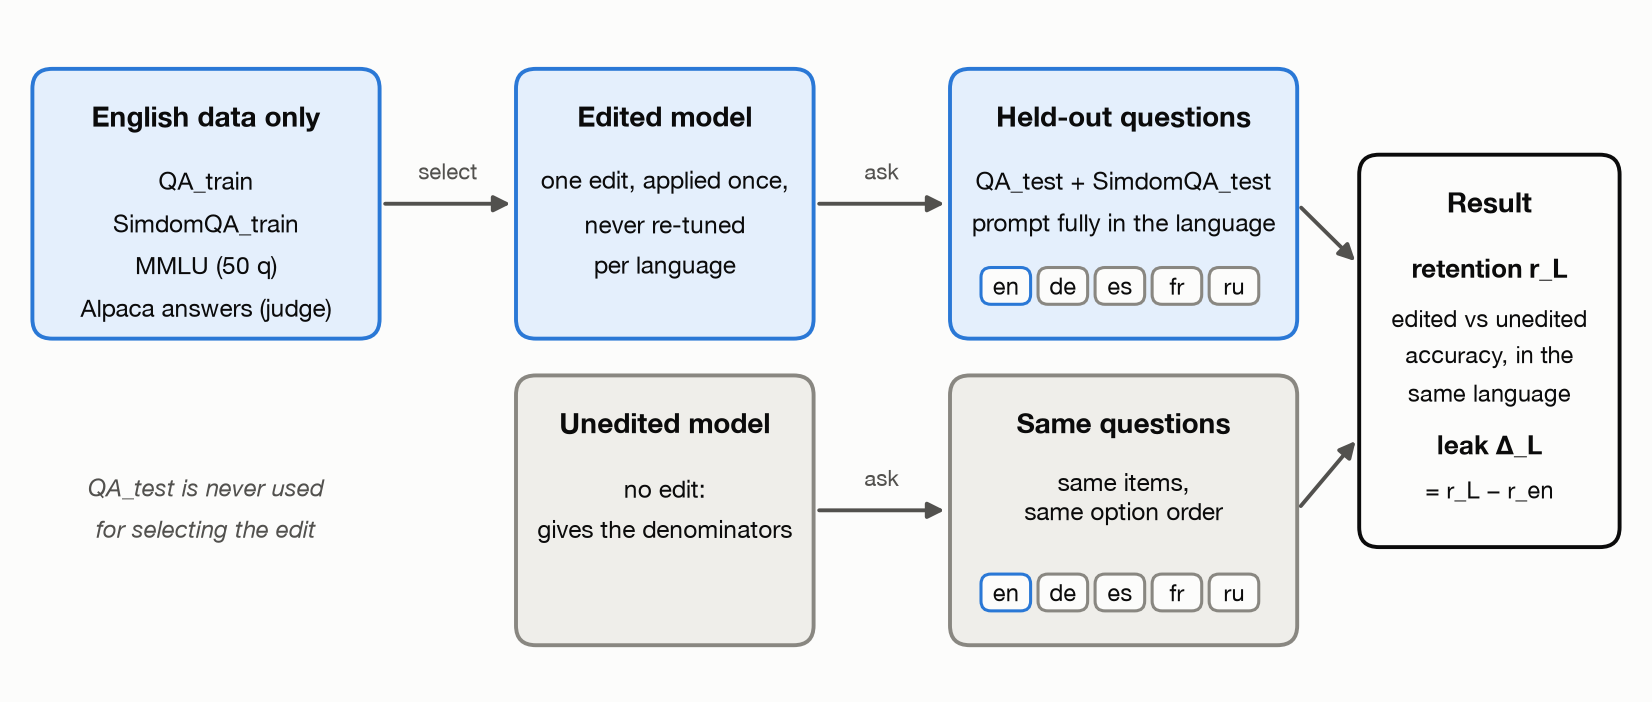
\includegraphics[width=0.92\textwidth]{fig0_protocol.png}
\caption{Cross-lingual evaluation protocol. The edit is selected on English data only (blue, top). The same edited model is then asked the held-out questions in five languages, and the unedited model is asked the same questions to provide the denominators (grey, bottom).}
\label{fig:1}
\end{figure*}

\subsection{Model, concepts and features}\label{sec:3.1}

We use Gemma-2-2B-it \citep{gemma2024gemma2} in bfloat16 with greedy decoding. The 18 concepts are those of the EMBER paper. Eleven come from \citet{gurarieh2025precise}: Ancient Rome, Baseball, Cannabis, Culture of Greece, Gambling, Golf, Gun, Harry Potter, Pornography, Republic of Ireland and Uranium. Seven come from ConceptVectors \citep{hong2025intrinsic}: Artificial intelligence, COVID-19 pandemic, Halloween, Heroin, Nazism, Valentine's Day and World War II. We use the features released with the EMBER paper for Gemma (rank $k=100$, seed 42), both the embedding features (EMBER) and the MLP features (SNMF), and we do not refit them. The edits are therefore exactly those of the paper at a given strength.

\subsection{Evaluation data}\label{sec:3.2}

Table~\ref{tab:1} lists the data. Every concept has 50 four-option multiple-choice (MC) questions for selecting the edit (\qatrain{}) and 50 disjoint held-out questions for evaluation (\qatest{}). Each concept also has 50 + 50 questions on a similar but different topic (\texttt{SimdomQA}), for example other fantasy novels for Harry Potter. These questions measure whether the edit damages neighbouring knowledge. General knowledge is measured with MMLU \citep{hendrycks2021mmlu}, and coherence with AlpacaEval prompts \citep{taori2023alpaca}.

\begin{table*}[t]
\centering\small
\begin{tabular}{@{}p{0.15\textwidth}p{0.36\textwidth}p{0.15\textwidth}p{0.25\textwidth}@{}}
\toprule
Set & Per concept & Languages & Used for \\
\midrule
\qatrain{} & 50 MC questions about the concept & English & selecting the edit (efficacy) \\
\qatest{} & 50 MC questions about the concept (disjoint from train) & en, de, es, fr, ru & held-out evaluation (retention, leak) \\
\simdomtrain{} & 50 MC questions on a similar but different topic & English & selecting the edit (specificity) \\
\simdomtest{} & 50 MC questions on the similar topic & en, de, es, fr, ru & collateral damage in each language \\
MMLU & 50 questions (selection) / 1,000 questions (test) & English & general knowledge \\
AlpacaEval prompts & 150 prompts; the first 50 answers are judged & English & coherence \\
\bottomrule
\end{tabular}
\caption{Data used in Part 1.}
\label{tab:1}
\end{table*}

There are 200 questions per concept and 3,600 per language, so the four translations add 14,400 questions. The questions and their options were machine-translated into German, Spanish, French and Russian with \texttt{gemini-3.5-flash-lite}, and were then corrected and validated with an automatic script and tool-assisted review (including a review by Claude).

\subsection{Erasure methods and hyperparameter grids}\label{sec:3.3}

Table~\ref{tab:2} lists the methods and their search spaces, which are those of the EMBER paper. The fixed settings (rank 100, 1\% sparsity, ratio threshold $\tau=2.0$, neuron-coverage threshold 0.95) are also those of the EMBER paper.

\begin{table*}[t]
\centering\small
\begin{tabular}{@{}p{0.12\textwidth}p{0.3\textwidth}p{0.4\textwidth}p{0.07\textwidth}@{}}
\toprule
Method & What is edited & Hyperparameters searched & Grid size \\
\midrule
EMBER & embedding rows of 31--86 concept tokens & $\delta\in\{0.5,1,2,5,10,50,100,200\}$ & 8 \\
SNMF & MLP input weights (\texttt{up\_\allowbreak{}proj}) and output weights (\texttt{down\_\allowbreak{}proj}) along concept features & $\delta_{\mathrm{in}},\delta_{\mathrm{out}}\in\{1,4,7,10\}$; input layers 0--8 / 0--12 / 0--25; output layers 0--8 / 9--17 / 13--25 & 144 \\
SNMF+EMBER & EMBER at the concept's selected $\delta$, then SNMF & SNMF grid on top of the fixed EMBER $\delta$ & 144 \\
\bottomrule
\end{tabular}
\caption{Methods and search spaces.}
\label{tab:2}
\end{table*}

\subsection{Coherence judge}\label{sec:3.4}

The EMBER paper scores AlpacaEval answers with Gemini, on instruction following and fluency (0--2 each). A full search over 18 concepts needs tens of thousands of judge calls, so we replaced Gemini with Qwen2.5-32B-Instruct \citep{qwen2024qwen25}, run locally in 4-bit (NF4) quantization \citep{dettmers2023qlora} on three 11 GB GPUs. We required the judge to come from a different model family than the erased model (Gemma), because a judge from the same family could share its blind spots, and to stay close to Gemini. To test the second requirement we re-judged Gemini's own 150 saved AlpacaEval answers item by item with Gemini's original prompts, and required the mean difference from Gemini to stay within $\pm$0.15 on both scores.

\begin{table*}[t]
\centering\small
\begin{tabular}{@{}lccc@{}}
\toprule
 & Qwen2.5-14B & \textbf{Qwen2.5-32B (chosen)} & Gemma-4-12B \\
\midrule
Instruction: mean diff. vs Gemini & $-$0.100 & \textbf{$-$0.073} & +0.013 \\
Instruction: exact match & 91.3\% & \textbf{92.7\%} & --- \\
Fluency: mean diff. vs Gemini & +0.200 (fails) & \textbf{+0.040} & +0.367 (fails) \\
Fluency: exact match & 61.3\% & 64.0\% & --- \\
Parse failures & 0 / 300 & 0 / 300 & --- \\
\bottomrule
\end{tabular}
\caption{Agreement with Gemini on the same 150 AlpacaEval answers (scores 0--2). The acceptance band for the mean difference is $\pm$0.15.}
\label{tab:3}
\end{table*}

Qwen2.5-32B passes both axes with Gemini's original, unmodified prompts. Qwen2.5-14B fails on fluency even with a prompt rewritten for it, and Gemma-4-12B fails on fluency and belongs to the same family as the erased model (Table~\ref{tab:3}). On individual answers the fluency agreement is only 64\%, but the disagreements go both ways and cancel in the mean. Our selection uses only means over 50 answers, so we use the judge only through means. With this judge the unedited model scores 1.927 (instruction following) and 1.687 (fluency) on the 150 selection prompts, and all selection scores are normalized by these values. Generation and judging are run as two separate passes, because the model being erased and the judge do not fit on the same GPU.

\subsection{Selecting a configuration (English only)}\label{sec:3.5}

Each (concept, method) pair gets exactly one edit, selected on English data only. In the first pass, no judge is used: every grid cell is applied and scored on \qatrain{}, \simdomtrain{} and the 50-question MMLU set, the cells are ranked by the judge-free score HM(efficacy, specificity) (Section~\ref{sec:4}), and the top three are kept. In the second pass, the first 50 AlpacaEval answers of each of the three candidates are judged with Qwen, and the cell with the highest full selection score HM(efficacy, specificity, coherence) is chosen. As in the original pipeline, a cell is discarded if its MMLU falls below 90\% of the unedited model on the chance-corrected scale. For EMBER, both judge scores must also stay at or above 90\% of the unedited model; SNMF and SNMF+EMBER have no judge gate.

We deviate from the original protocol in two ways. First, the EMBER paper judges the top 15 cells on 150 answers for SNMF and all 8 cells on 150 answers for EMBER. For computational reasons we judge fewer cells and fewer answers: a single judge call took about 30 seconds, and only part of the available nodes can host the judge model. We nevertheless kept the logic of the grid search and did not drop the coherence test.

Second, we changed how multiple-choice answers are read. Gemma should answer a closed question with a single letter, but it sometimes answers with a sentence (``The answer is ...''). The original scorer generates only four new tokens, so such an answer is cut off before the letter and counted as wrong. We regard this as a failure to follow the answer format, not as evidence that the concept was erased, and we therefore allow 32 new tokens and use a stricter letter parser. Without this change EMBER would look stronger, since an answer that is cut off counts as if the model had forgotten the concept. All selections and evaluations in this report use the corrected scorer.

\section{Metrics}\label{sec:4}

\textbf{Accuracy and normalization.} We use four-option multiple-choice (MC) accuracy, scored with greedy decoding and no judge, so the score is identical in every language. Unparseable answers count as wrong. As in \citet{suslik2026ember}, accuracies are normalized against the unedited model and corrected for the 0.25 chance level:

\begin{equation*}
\phi(a;a_0)=\operatorname{clip}\!\left(\frac{a-0.25}{a_0-0.25},\,0,\,1\right),
\end{equation*}

where $a$ is the edited and $a_0$ the unedited accuracy. A value of 1 means unchanged and 0 means chance.

\textbf{Selection metrics (English).} We follow the EMBER paper without change, except for the judge:

\begin{itemize}
\setlength\itemsep{1pt}
\item efficacy $=1-\phi(\text{QA}_{\text{train}})$;
\item specificity $=\operatorname{HM}\big(\phi(\text{MMLU}),\,\phi(\text{SimDom}_{\text{train}})\big)$, which covers general and neighbouring-topic damage;
\item coherence $=\operatorname{HM}$ of the AlpacaEval instruction-following and fluency scores, each divided by the unedited model's score and capped at 1;
\item selection score $H=\operatorname{HM}(\text{efficacy},\text{specificity},\text{coherence})$.
\end{itemize}

The harmonic mean ($\operatorname{HM}$) is dominated by its smallest term, so an edit cannot score well by breaking one axis. We use the paper's gates (MMLU fraction $\ge 0.9$; for EMBER also both judge fractions $\ge 0.9$). Because Gemini is paid, coherence is scored by Qwen2.5-32B-Instruct instead (Section~\ref{sec:3.4}). The first selection pass ranks cells by the judge-free $\operatorname{HM}(\text{efficacy},\text{specificity})$ and the second pass judges only the top three.

\textbf{Retention and leak (cross-lingual).} For language $L$, on the held-out $\text{QA}_{\text{test}}$,

\begin{equation*}
r_L=\phi\big(\mathrm{acc}_L;\ \mathrm{acc}^{\text{unedited}}_L\big),\qquad \Delta_L=r_L-r_{\text{en}}.
\end{equation*}

Lower $r_L$ means stronger erasure, and $\Delta_L>0$ means the concept survives better in $L$ than in English. The paper has no cross-lingual measure, so both are ours. We normalize by the unedited accuracy \emph{in the same language} because Gemma knows less in Russian (0.52) than in English (0.73), and only the per-language ratio separates ``erased'' from ``never known''. We report $\Delta_L$ as a difference rather than a ratio because $r_{\text{en}}$ can be near 0. A concept--language pair is dropped when the unedited accuracy is below 0.40 (2 of 90 pairs), since with 50 questions the denominator is then mostly noise. The mean leak averages a concept's reliable languages first, then concepts.

\textbf{Collateral damage.} $\phi$ on $\text{SimDom}_{\text{test}}$ in each language, and English MMLU accuracy on the 1,000-question test split. MMLU is not translated, so specificity in a language is in-language SimDom plus English MMLU.

\textbf{Invalid answers.} We report the share of unparseable answers per language next to retention, because a broken answer is scored as wrong and so looks like erasure (Table~\ref{tab:5}).

\textbf{Statistics.} The unit of analysis is the concept. We report 95\% bootstrap intervals over concepts (10,000 resamples) and compare methods by paired per-concept differences with a bootstrap interval and a paired $t$-test.

\section{Results}\label{sec:5}

\subsection{English selection}\label{sec:5.1}

Table~\ref{tab:4} and Figure~\ref{fig:2} summarize the edits selected for each method; per-concept picks are in Appendix~\ref{app:B}. These scores are measured on the English selection data. Since each edit is the best of 8 (EMBER) or 144 (SNMF and SNMF+EMBER) candidates on the same questions, they are optimistic, and the held-out results in Section~\ref{sec:5.2} are the reliable ones.

SNMF+EMBER reaches the highest selection score (0.888) and is the best method for 17 of 18 concepts; Harry Potter is the exception, where SNMF scores higher (0.929 against 0.903). SNMF follows (0.820) and EMBER is last (0.667). The ordering is driven by efficacy: EMBER erases less than half of the concept on average (efficacy 0.43), against 0.72 for SNMF and 0.83 for SNMF+EMBER. In exchange, EMBER is the most specific (0.970) and the most coherent (0.992), because it edits only 31--86 tokens per concept, whereas SNMF (specificity 0.848) and SNMF+EMBER (0.892) lose more neighbouring and general knowledge.

\begin{figure}[t]
\centering
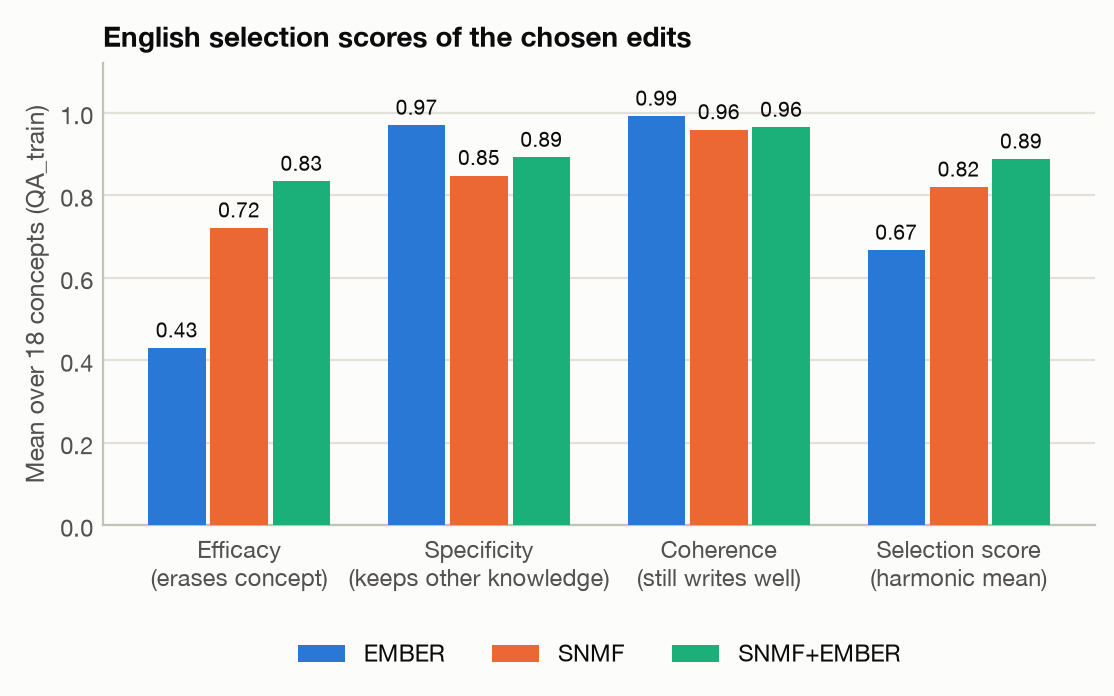
\includegraphics[width=\columnwidth]{fig2_selection_scores.png}
\caption{Mean selection metrics of the 18 chosen edits, measured on the selection data (\qatrain{}, \simdomtrain{}, MMLU-50, 50 judged AlpacaEval answers).}
\label{fig:2}
\end{figure}

\begin{table*}[t]
\centering\small
\begin{tabular}{@{}lccccl@{}}
\toprule
Method & Efficacy & Specificity & Coherence & Selection score & Best on \\
\midrule
EMBER & 0.430 (0.403) & \textbf{0.970} (0.965) & \textbf{0.992} (0.998) & 0.667 (0.661) & 0 / 18 \\
SNMF & 0.721 (0.698) & 0.848 (0.858) & 0.959 (0.962) & 0.820 (0.833) & 1 / 18 (Harry Potter) \\
SNMF+EMBER & \textbf{0.834} (0.847) & 0.892 (0.891) & 0.965 (0.974) & \textbf{0.888} (0.896) & \textbf{17 / 18} \\
\bottomrule
\end{tabular}
\caption{Selection results, mean over 18 concepts (median in brackets).}
\label{tab:4}
\end{table*}

Figure~\ref{fig:3} shows why EMBER cannot simply be pushed harder. With the corrected scorer, efficacy rises quickly up to $\delta \approx 10$ and then plateaus at 0.34--0.38 (Figure~\ref{fig:3}b), so stronger edits do not erase more. The original four-token scorer suggested the opposite: concept accuracy kept falling for $\delta \geq 50$ (Figure~\ref{fig:3}a), because answers such as ``The answer is \textbf{C}'' were cut off before the letter and counted as wrong. At $\delta = 100$ about 11\% of the answers were affected. EMBER's AlpacaEval answers also hardly depend on $\delta$: for every $\delta$ we judged, 48--50 of the 50 answers were identical to those at another $\delta$ of the same concept, since everyday prompts rarely contain the edited tokens. The choice of $\delta$ is therefore decided by efficacy and specificity.

\begin{figure*}[t]
\centering
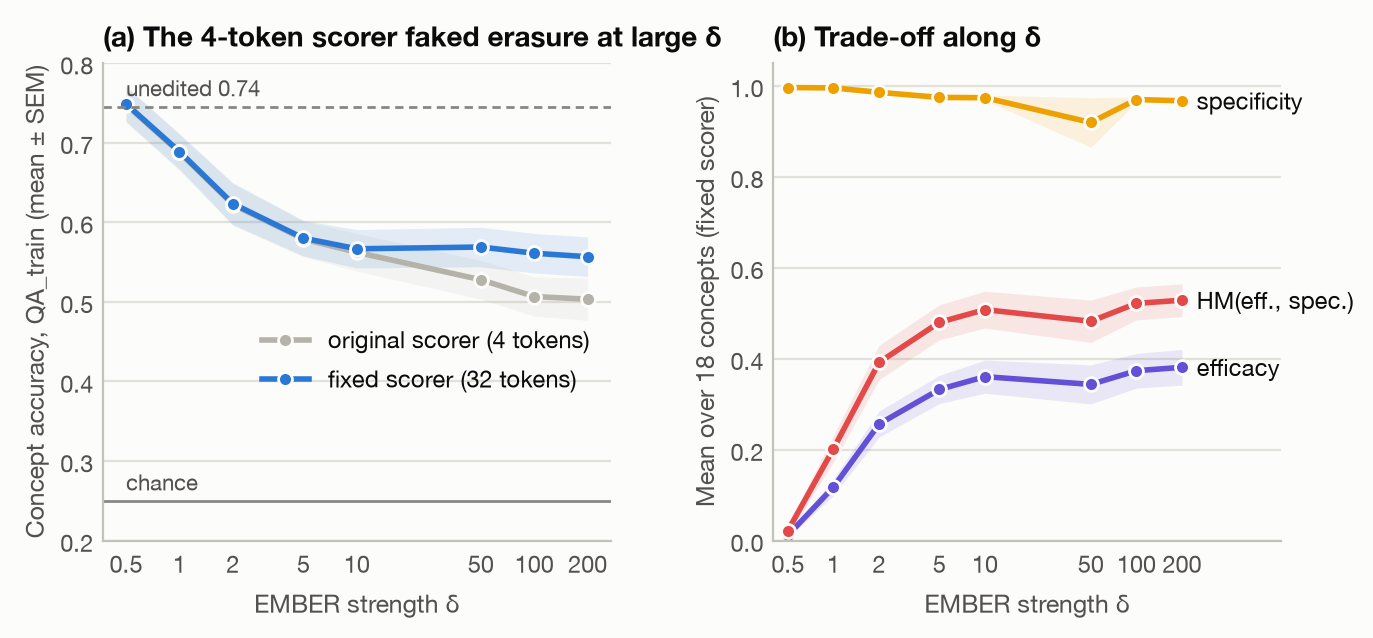
\includegraphics[width=0.85\textwidth]{fig3_ember_delta_sweep.png}
\caption{EMBER across its eight strengths, mean $\pm$ SEM over 18 concepts. (a) Concept accuracy with the original four-token scorer and the corrected scorer. (b) Efficacy, specificity and the judge-free score with the corrected scorer.}
\label{fig:3}
\end{figure*}

\subsection{Cross-lingual transfer}\label{sec:5.2}

Figures~\ref{fig:4} and~\ref{fig:5} and Table~\ref{tab:5} report retention and leak on the held-out \qatest{} questions, with every edit selected in English only. Single (concept, language) cells are noisy, since each has only 50 questions and the leak of one cell has a standard deviation of roughly 0.2--0.3. We therefore draw conclusions only from averages over concepts; per-concept values are in Appendix~\ref{app:C}.

EMBER erases English only partially (retention 0.61) and erases less in every other language: retention is 0.71 in German, 0.81 in Spanish, 0.76 in French and 0.96 in Russian, where the model is almost indistinguishable from the unedited one. The mean leak is +0.19 (95\% CI [+0.11, +0.27]), the interval of each individual language excludes zero, and 16 of 18 concepts leak on average. The order of the languages is consistent with an account in which the embedding edit only reaches questions that share tokens with the English concept words: German, Spanish and French keep many names and technical terms in Latin script, whereas Russian writes them in Cyrillic (Section~\ref{sec:6}).

SNMF erases about equally in all languages: retention lies between 0.43 and 0.51 everywhere. Every per-language interval contains zero, the mean leak is +0.01 ([$-$0.07, +0.08]), and only 9 of 18 concepts have a positive mean leak, so a mean leak above roughly 0.08 is unlikely. The intervals of EMBER and SNMF do not overlap.

SNMF+EMBER has the lowest English retention of the three (0.39), although its interval overlaps that of SNMF (0.45). Its leak into German, Spanish and French is indistinguishable from zero, and its mean leak is +0.04 ([$-$0.02, +0.11]). Russian, however, still leaks (+0.23, [+0.08, +0.38]; retention 0.64). Both methods that contain the EMBER edit therefore leak into Russian, the only tested language with a non-Latin script, whereas SNMF alone does not (+0.05, [$-$0.06, +0.15]). After the scorer correction, unparseable answers are rare, at most 2.2\% per language on average (Table~\ref{tab:5}), and count as wrong.

\begin{figure}[t]
\centering
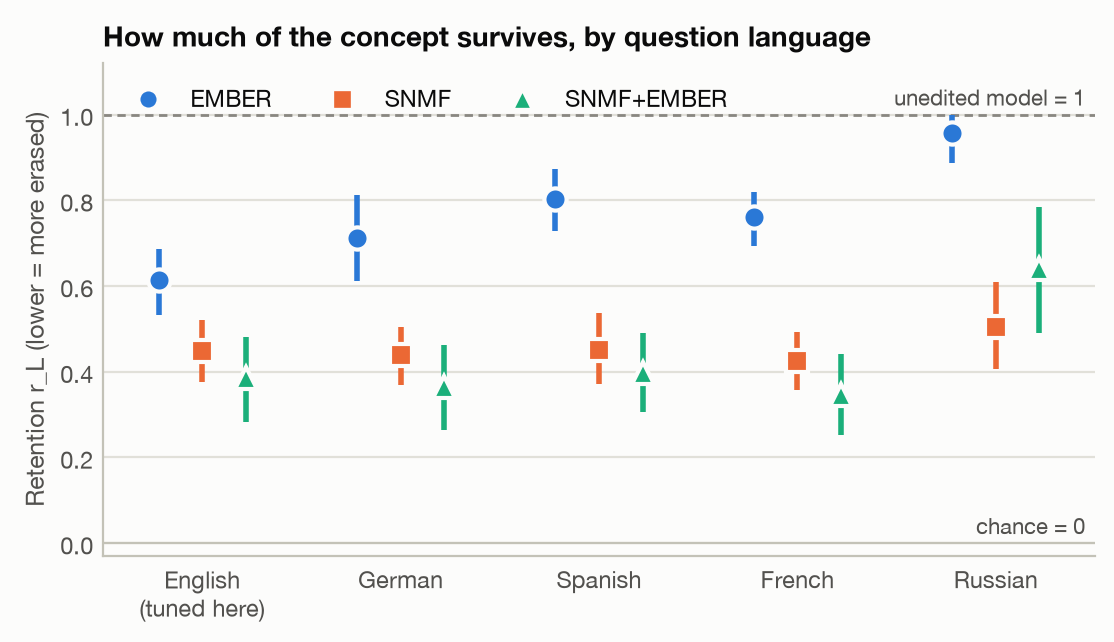
\includegraphics[width=\columnwidth]{fig4_retention_by_language.png}
\caption{Retention $r_L$ per question language (lower = more erased; 1 = unedited, 0 = chance). Mean over concepts with 95\% bootstrap intervals (18 concepts; 16 for Russian). Every edit was tuned in English only.}
\label{fig:4}
\end{figure}

\begin{figure}[t]
\centering
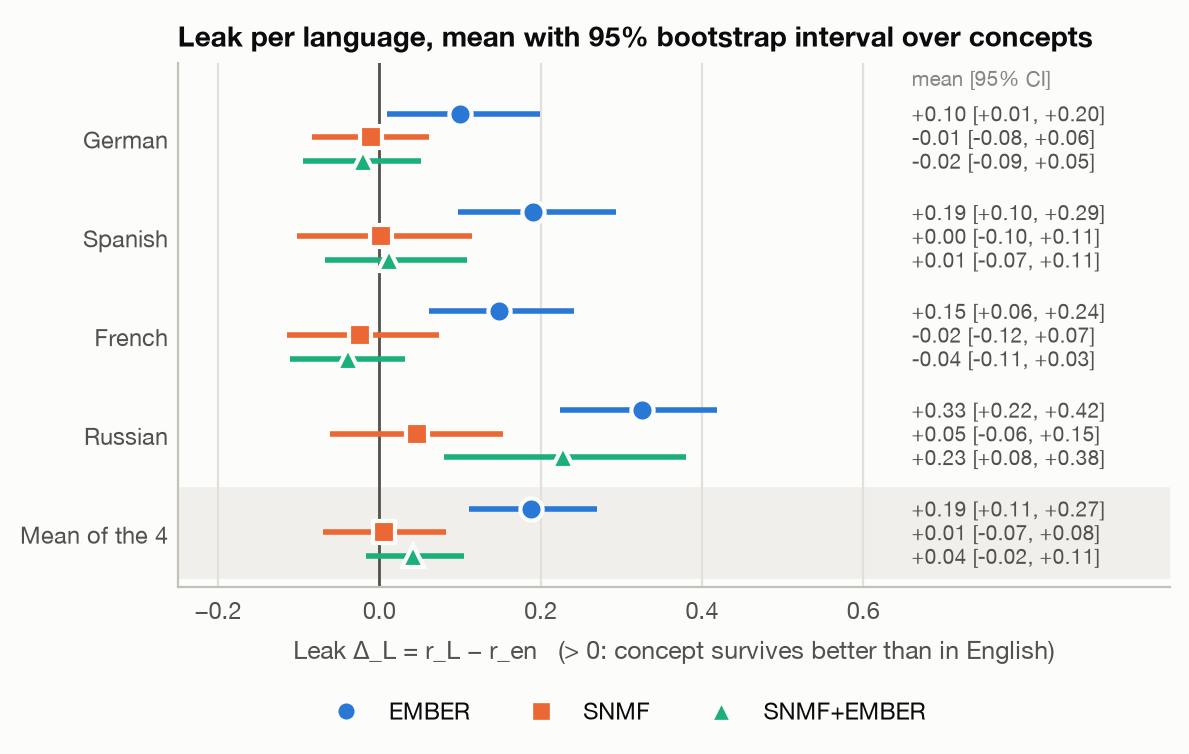
\includegraphics[width=\columnwidth]{fig5_leak_by_language.png}
\caption{Leak $\Delta_L=r_L-r_{\mathrm{en}}$ per language and averaged over the four languages, with 95\% bootstrap intervals. An interval that does not cross the vertical zero line indicates a reliable leak.}
\label{fig:5}
\end{figure}

\begin{table*}[t]
\centering\small
\begin{tabular}{@{}lccc@{}}
\toprule
 & EMBER & SNMF & SNMF+EMBER \\
\midrule
English \qatest{} accuracy (unedited 0.73) & 0.55 & 0.47 & \textbf{0.44} \\
Retention $r_{\mathrm{en}}$ / $r_{\mathrm{de}}$ / $r_{\mathrm{es}}$ / $r_{\mathrm{fr}}$ / $r_{\mathrm{ru}}$ & 0.61 / 0.71 / 0.81 / 0.76 / \textbf{0.96} & 0.45 / 0.44 / 0.45 / 0.43 / 0.51 & \textbf{0.39} / 0.37 / 0.40 / 0.35 / 0.64 \\
Leak $\Delta_{\mathrm{de}}$ & \textbf{+0.10} [+0.01, +0.20] & $-$0.01 [$-$0.08, +0.06] & $-$0.02 [$-$0.09, +0.05] \\
Leak $\Delta_{\mathrm{es}}$ & \textbf{+0.19} [+0.10, +0.29] & +0.00 [$-$0.10, +0.11] & +0.01 [$-$0.07, +0.11] \\
Leak $\Delta_{\mathrm{fr}}$ & \textbf{+0.15} [+0.06, +0.24] & $-$0.02 [$-$0.11, +0.07] & $-$0.04 [$-$0.11, +0.03] \\
Leak $\Delta_{\mathrm{ru}}$ & \textbf{+0.33} [+0.22, +0.42] & +0.05 [$-$0.06, +0.15] & \textbf{+0.23} [+0.08, +0.38] \\
Mean leak over de/es/fr/ru & \textbf{+0.19} [+0.11, +0.27] & +0.01 [$-$0.07, +0.08] & +0.04 [$-$0.02, +0.11] \\
Concepts with mean leak > 0 & 16 / 18 & 9 / 18 & 11 / 18 \\
Invalid answers, en / mean of the others & 0.006 / 0.006 & 0.000 / 0.000 & 0.018 / 0.016 \\
\bottomrule
\end{tabular}
\caption{Cross-lingual results on the held-out \qatest{} (95\% bootstrap interval over concepts in brackets).}
\label{tab:5}
\end{table*}

Bold leak values have an interval that excludes 0. The mean leak first averages each concept over its reliable languages; averaging the four per-language means instead gives +0.19 / +0.00 / +0.05, with the same conclusions.

\subsection{Collateral damage}\label{sec:5.3}

Figure~\ref{fig:6} and Table~\ref{tab:6} show what the edits cost. EMBER is the most precise: it retains 95--100\% of the similar-domain knowledge in every language, and English MMLU stays at 0.547 against 0.553 for the unedited model. SNMF and SNMF+EMBER are much broader. They retain only 59--76\% of the similar-domain knowledge in every language, and English MMLU falls to 0.506 and 0.507. Some concepts are hit much harder, for example Valentine's Day under SNMF (MMLU 0.442) and COVID-19 under SNMF+EMBER (0.439).

The lack of a leak for SNMF should therefore not be read as a clean erasure. Its edit removes the concept together with part of its neighbours and of general knowledge, in all languages, whereas EMBER is precise but reaches only the English tokens. No method combines a low leak with low collateral damage (Figure~\ref{fig:7}). The selection could not have prevented the MMLU loss, because it uses only 50 MMLU questions: their standard error of about 0.07 hides a drop of 0.05, and a larger MMLU set or a constraint on SimDom would be needed. The damage is not an artifact of our judge or selection policy. For the eight concepts shared with our earlier pilot with a Gemini judge, five of the eight selected SNMF edits are identical, and the new edits are on average slightly less damaging (Appendix~\ref{app:D}).

\begin{figure*}[t]
\centering
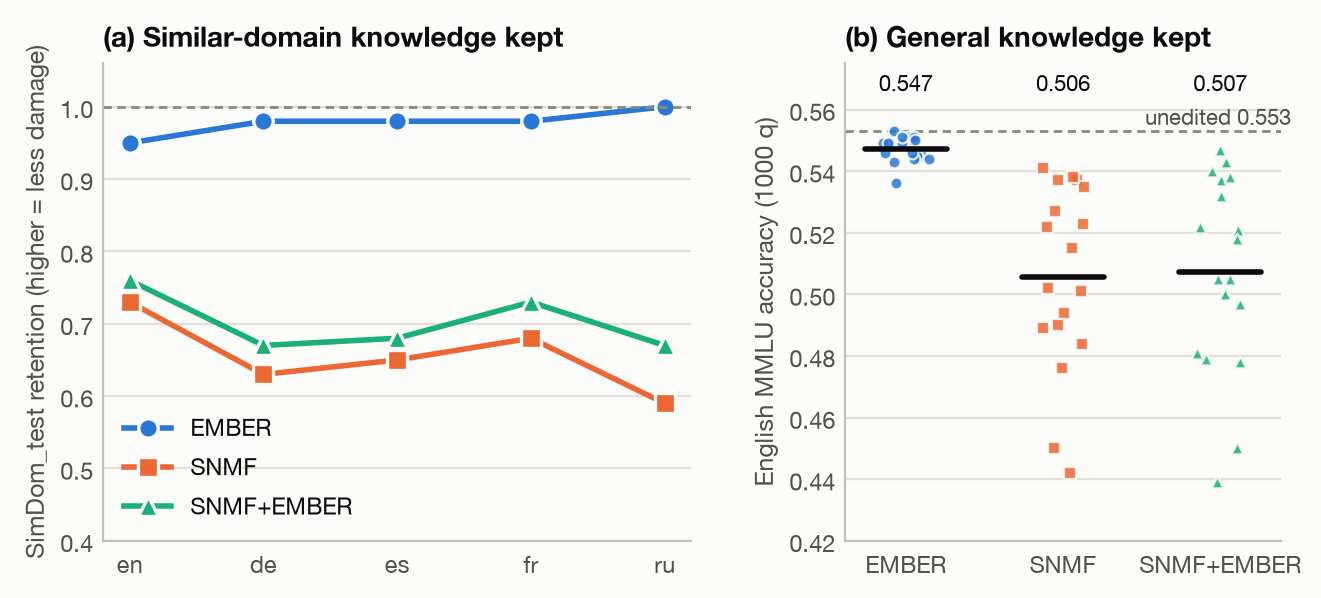
\includegraphics[width=0.85\textwidth]{fig6_collateral_damage.png}
\caption{(a) Similar-domain retention per language (higher = less damage). (b) English MMLU on 1,000 questions, one dot per concept (horizontal bar = mean; dashed line = unedited).}
\label{fig:6}
\end{figure*}

\begin{table*}[t]
\centering\small
\begin{tabular}{@{}lccc@{}}
\toprule
 & EMBER & SNMF & SNMF+EMBER \\
\midrule
\simdomtest{} accuracy, en (unedited 0.89) & \textbf{0.87} & 0.73 & 0.75 \\
\simdomtest{} accuracy, mean non-en (unedited 0.73) & \textbf{0.73} & 0.57 & 0.59 \\
SimDom retention, en / de / es / fr / ru & \textbf{0.95 / 0.98 / 0.98 / 0.98 / 1.00} & 0.73 / 0.63 / 0.65 / 0.68 / 0.59 & 0.76 / 0.67 / 0.68 / 0.73 / 0.67 \\
English MMLU, 1,000 q (unedited 0.553), mean (min--max) & \textbf{0.547} (0.536--0.553) & 0.506 (0.442--0.541) & 0.507 (0.439--0.547) \\
\bottomrule
\end{tabular}
\caption{Collateral damage of the selected edits.}
\label{tab:6}
\end{table*}

\begin{figure}[t]
\centering
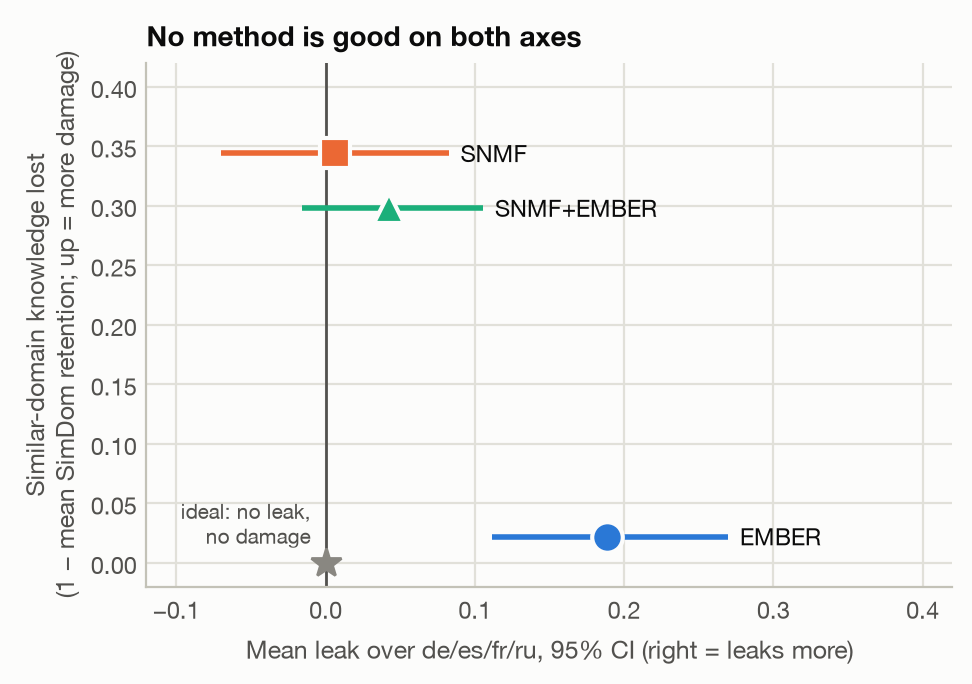
\includegraphics[width=0.9\columnwidth]{fig7_tradeoff.png}
\caption{Mean leak (x, with 95\% CI) against similar-domain knowledge lost (y). The ideal edit sits at the star (no leak, no damage).}
\label{fig:7}
\end{figure}

\subsection{Comparison with the EMBER paper}\label{sec:5.4}

Table~\ref{tab:7} compares our English held-out results with Table 1 of the EMBER paper. With the original scorer our results are close to the paper's: concept accuracy is 0.50 against 0.494 for EMBER and 0.38 against 0.377 for SNMF+EMBER, and the similar-domain and MMLU accuracies agree within about 0.03. This holds although we replaced the judge and judged fewer cells, which supports the view that our pipeline reproduces the original one. With the corrected scorer the embedding-based methods erase less (EMBER 0.55, SNMF+EMBER 0.44), while SNMF is unchanged (0.47). The evaluator in the paper's released code also generates four tokens, so its EMBER numbers may be affected in the same way; we cannot verify this without the paper's raw outputs. The ranking of the methods is the same as in the paper: SNMF+EMBER erases the most and EMBER is the most specific.

\begin{table*}[t]
\centering\small
\begin{tabular}{@{}lccc@{}}
\toprule
 & Paper & Ours, original scorer & Ours, corrected scorer \\
\midrule
\textbf{Concept accuracy} ($\downarrow$), unedited & 0.733 & 0.73 & 0.73 \\
EMBER & 0.494 & 0.50 & 0.55 \\
SNMF & 0.437 & 0.47 & 0.47 \\
SNMF+EMBER & 0.377 & 0.38 & 0.44 \\
\midrule
\textbf{Similar-domain accuracy} ($\uparrow$), unedited & 0.892 & 0.89 & 0.89 \\
EMBER & 0.864 & 0.87 & 0.87 \\
SNMF & 0.699 & 0.73 & 0.73 \\
SNMF+EMBER & 0.778 & 0.78 & 0.75 \\
\midrule
\textbf{MMLU} ($\uparrow$), unedited & 0.542 & 0.553 & 0.553 \\
EMBER & 0.537 & 0.548 & 0.547 \\
SNMF & 0.484 & 0.506 & 0.506 \\
SNMF+EMBER & 0.510 & 0.511 & 0.507 \\
\bottomrule
\end{tabular}
\caption{Our English held-out results next to the paper's (Gemma-2-2B-it, multiple choice; the paper's Table 1 values are divided by 100). The multiple-choice evaluator in the paper's released code is the original four-token scorer.}
\label{tab:7}
\end{table*}

\section{Discussion}\label{sec:6}

The embedding edit does not travel well across languages. EMBER changes about 57 English token rows per concept, so a question in another language reaches the concept only through the tokens it shares with English. The ordering of the leak supports this. German, Spanish and French, which often keep names and terms in Latin script (e.g. \emph{Expelliarmus}), leak moderately (+0.10 to +0.19). Russian, which transliterates them (\emph{\cyr{Экспеллиармус}}), leaks the most (+0.33, retention 0.96). Our design does not prove that token overlap is the cause, since we did not count the edited tokens per question here, but it is the simplest explanation consistent with all three methods: the only method without an embedding edit, SNMF, is also the only one without a Russian leak.

The MLP edit transfers, at a price. SNMF's erasure is the same in every language, which matches the view that much of a model's knowledge passes through shared, language-independent representations in the middle layers. However, SNMF on this grid is a broad edit: it also removes about a third of the knowledge on neighbouring topics and about five MMLU points, so its absence of a leak is partly an absence of precision.

SNMF+EMBER inherits both properties. It erases English the most; its SNMF part erases in all languages, so German, Spanish and French show no leak, while its EMBER part adds erasure for English and Latin-script languages that Russian does not receive, so Russian leaks (+0.23). In practice, an erasure that is tuned and checked only in English can look successful and still leave the concept accessible in another language, especially one with a different script. Erasure evaluations should therefore include at least one non-Latin-script language, and embedding-based erasure needs multilingual concept tokens, which is the topic of Part 2.

Finally, a scoring detail, the four-token answer budget, changed the size of every effect and reversed one conclusion. Erasure that makes the model answer in sentences instead of letters looks like forgetting to a strict scorer, so the share of unparseable answers should be reported and the raw outputs should be read.

\subsection{Limitations}

\begin{enumerate}
\setlength\itemsep{1pt}
\item \textbf{One model, one feature seed.} We use only Gemma-2-2B-it with the released rank-100, seed-42 features. The EMBER paper also covers Llama-3.1-8B.
\item \textbf{Multiple choice only.} Open-ended answers in translated languages were too weak at baseline to measure.
\item \textbf{50 questions per cell and machine translation.} Single cells are noisy, and translations may differ in difficulty despite the aligned option order. Our bootstrap intervals do not include translation uncertainty.
\item \textbf{The metric is clipped.} Concepts erased to chance in English can only show a positive leak.
\item \textbf{Mixed specificity.} It combines in-language SimDom with English-only MMLU.
\item \textbf{No cross-lingual relearning test}, which is the main robustness test of the paper.
\item \textbf{Multiple testing.} The per-language comparisons are not corrected for multiple tests.
\item \textbf{Remaining invalid answers} (at most 2.2\% per language on average) are real non-answers (empty output, loops) and count as wrong.
\end{enumerate}

\section{Conclusion}\label{sec:7}

On Gemma-2-2B-it, across 18 concepts and five languages, an erasure tuned in English does not transfer equally to all languages. EMBER, which edits English token embeddings, leaves the concept more intact in every other language and almost fully intact in Russian (mean leak +0.19; Russian +0.33). SNMF, which edits MLP weights, erases evenly across languages, but it also damages similar-domain and general knowledge. SNMF+EMBER erases English the most and leaks only into Russian. Correcting an answer-truncation problem in the scorer reduced EMBER's apparent erasure and leak and removed most of SNMF+EMBER's apparent general leak, while EMBER's leak and the Russian leak of both embedding-based methods survived the correction. These results motivate Part 2: extending embedding-based erasure to multilingual tokens.

\bibliography{../references}
\bibliographystyle{../acl_natbib}

\appendix
\renewcommand{\thetable}{\Alph{section}\arabic{table}}

\section{Unedited \qatest{} accuracy per concept and language}\label{app:A}
\setcounter{table}{0}

\begin{table}[t]
\centering\small
\resizebox{\columnwidth}{!}{%
\begin{tabular}{@{}lccccc@{}}
\toprule
Concept & en & de & es & fr & ru \\
\midrule
Ancient Rome & 0.80 & 0.58 & 0.68 & 0.64 & 0.48 \\
Artificial intelligence & 0.80 & 0.78 & 0.76 & 0.78 & 0.68 \\
Baseball & 0.66 & 0.62 & 0.60 & 0.56 & 0.48 \\
COVID-19 pandemic & 0.64 & 0.54 & 0.54 & 0.52 & 0.44 \\
Cannabis & 0.94 & 0.88 & 0.90 & 0.80 & 0.66 \\
Culture of Greece & 0.62 & 0.52 & 0.62 & 0.54 & 0.52 \\
Gambling & 0.84 & 0.80 & 0.76 & 0.70 & 0.58 \\
Golf & 0.80 & 0.76 & 0.72 & 0.72 & 0.50 \\
Gun & 0.82 & 0.66 & 0.64 & 0.62 & 0.66 \\
Halloween & 0.60 & 0.48 & 0.48 & 0.48 & 0.48 \\
Harry Potter & 0.80 & 0.60 & 0.58 & 0.50 & 0.36$^{*}$ \\
Heroin & 0.68 & 0.52 & 0.46 & 0.46 & 0.50 \\
Nazism & 0.74 & 0.70 & 0.72 & 0.66 & 0.50 \\
Pornography & 0.82 & 0.86 & 0.76 & 0.76 & 0.70 \\
Republic of Ireland & 0.74 & 0.66 & 0.54 & 0.58 & 0.48 \\
Uranium & 0.62 & 0.56 & 0.50 & 0.52 & 0.46 \\
Valentine's Day & 0.46 & 0.44 & 0.44 & 0.42 & 0.32$^{*}$ \\
World War II & 0.74 & 0.64 & 0.62 & 0.62 & 0.48 \\
\midrule
\textbf{Mean} & \textbf{0.73} & \textbf{0.64} & \textbf{0.63} & \textbf{0.60} & \textbf{0.52} \\
\bottomrule
\end{tabular}
}
\caption{Unedited \qatest{} accuracy per concept and language. A star marks a cell below the 0.40 screen (dropped).}
\end{table}

\section{Selected edits per concept (English selection data)}\label{app:B}
\setcounter{table}{0}

\begin{table*}[t]
\centering\small
\begin{tabular}{@{}lccccccc@{}}
\toprule
Concept & $\delta$ & Features & Tokens & Efficacy & Specificity & Coherence & Score \\
\midrule
Ancient Rome & 200 & 3 & 86 & 0.618 & 0.947 & 0.998 & 0.816 \\
Artificial intelligence & 100 & 2 & 59 & 0.211 & 1.000 & 0.966 & 0.442 \\
Baseball & 200 & 3 & 79 & 0.203 & 0.925 & 0.992 & 0.428 \\
COVID-19 pandemic & 50 & 1 & 42 & 0.364 & 0.986 & 0.998 & 0.630 \\
Cannabis & 200 & 1 & 45 & 0.305 & 1.000 & 0.992 & 0.568 \\
Culture of Greece & 200 & 1 & 52 & 0.857 & 0.969 & 1.000 & 0.938 \\
Gambling & 10 & 3 & 69 & 0.471 & 0.962 & 0.998 & 0.720 \\
Golf & 10 & 2 & 70 & 0.407 & 1.000 & 0.992 & 0.672 \\
Gun & 5 & 2 & 61 & 0.407 & 0.935 & 1.000 & 0.663 \\
Halloween & 10 & 2 & 80 & 0.400 & 0.962 & 0.990 & 0.659 \\
Harry Potter & 10 & 1 & 39 & 0.526 & 1.000 & 0.990 & 0.767 \\
Heroin & 100 & 1 & 46 & 0.564 & 1.000 & 0.998 & 0.795 \\
Nazism & 100 & 1 & 41 & 0.549 & 0.940 & 0.998 & 0.772 \\
Pornography & 5 & 1 & 43 & 0.327 & 1.000 & 0.998 & 0.592 \\
Republic of Ireland & 100 & 1 & 31 & 0.326 & 0.984 & 0.998 & 0.589 \\
Uranium & 200 & 2 & 70 & 0.359 & 0.962 & 0.998 & 0.621 \\
Valentine's Day & 200 & 2 & 71 & 0.439 & 0.934 & 0.962 & 0.684 \\
World War II & 5 & 1 & 36 & 0.400 & 0.956 & 0.992 & 0.659 \\
\midrule
\textbf{Mean} &  & 1.7 & 57 & \textbf{0.430} & \textbf{0.970} & \textbf{0.992} & \textbf{0.667} \\
\bottomrule
\end{tabular}
\caption{EMBER. ``Features'' = embedding features selected for the concept. ``Tokens'' = vocabulary rows edited.}
\end{table*}

The paper reports 1.7 embedding features per concept on average for Gemma, the same as ours.

\begin{table*}[t]
\centering\small
\resizebox{\textwidth}{!}{%
\begin{tabular}{@{}lllcccc@{}}
\toprule
Concept & $\delta_{\mathrm{in}}$ & $\delta_{\mathrm{out}}$ & Efficacy & Specificity & Coherence & Score \\
\midrule
Ancient Rome$^{1}$ & 7 @ 0--8 (k=13) & 1 @ 9--17 (k=4) & 0.618 & 0.934 & 0.948 & 0.802 \\
Artificial intelligence & 4 @ 0--25 (k=51) & 4 @ 0--8 (k=36) & 0.691 & 0.957 & 0.993 & 0.857 \\
Baseball & 1 @ 0--12 (k=33) & 10 @ 0--8 (k=29) & 0.702 & 0.771 & 0.998 & 0.806 \\
COVID-19 pandemic & 7 @ 0--8 (k=31) & 4 @ 9--17 (k=13) & 0.788 & 0.772 & 0.980 & 0.837 \\
Cannabis & 4 @ 0--8 (k=25) & 4 @ 0--8 (k=25) & 0.508 & 0.788 & 0.970 & 0.703 \\
Culture of Greece & 1 @ 0--25 (k=14) & 10 @ 0--8 (k=10) & 0.694 & 0.919 & 0.975 & 0.844 \\
Gambling & 10 @ 0--12 (k=26) & 7 @ 9--17 (k=6) & 0.863 & 0.808 & 0.939 & 0.867 \\
Golf & 4 @ 0--25 (k=35) & 7 @ 13--25 (k=10) & 0.590 & 0.887 & 0.879 & 0.758 \\
Gun & 4 @ 0--8 (k=36) & 4 @ 9--17 (k=4) & 0.852 & 0.806 & 0.955 & 0.867 \\
Halloween & 10 @ 0--12 (k=16) & 7 @ 13--25 (k=8) & 0.606 & 0.873 & 0.986 & 0.787 \\
Harry Potter & 7 @ 0--12 (k=16) & 1 @ 0--8 (k=15) & 0.877 & 0.919 & 0.998 & 0.929 \\
Heroin & 7 @ 0--25 (k=32) & 10 @ 9--17 (k=3) & 0.667 & 0.958 & 0.972 & 0.840 \\
Nazism & 10 @ 0--12 (k=25) & 1 @ 9--17 (k=9) & 0.980 & 0.608 & 0.942 & 0.805 \\
Pornography & 4 @ 0--8 (k=23) & 10 @ 9--17 (k=7) & 0.776 & 0.947 & 0.887 & 0.864 \\
Republic of Ireland & 1 @ 0--25 (k=9) & 10 @ 0--8 (k=5) & 0.558 & 0.826 & 0.952 & 0.740 \\
Uranium & 10 @ 0--25 (k=36) & 1 @ 0--8 (k=17) & 0.513 & 0.844 & 0.948 & 0.716 \\
Valentine's Day & 1 @ 0--12 (k=14) & 10 @ 0--8 (k=13) & 0.829 & 0.955 & 0.955 & 0.909 \\
World War II & 10 @ 0--25 (k=15) & 1 @ 13--25 (k=3) & 0.873 & 0.685 & 0.988 & 0.829 \\
\midrule
\textbf{Mean} &  &  & \textbf{0.721} & \textbf{0.848} & \textbf{0.959} & \textbf{0.820} \\
\bottomrule
\end{tabular}
}
\caption{SNMF. Notation: $\delta$ @ layers ($k$ = number of MLP features); ``in'' = \texttt{up\_\allowbreak{}proj}, ``out'' = \texttt{down\_\allowbreak{}proj}.}
\end{table*}

$^{1}$ Picked after a screen for looping answers: grid rank 9, the first healthy cell.

\begin{table*}[t]
\centering\small
\resizebox{\textwidth}{!}{%
\begin{tabular}{@{}llllcccc@{}}
\toprule
Concept & $\delta_{\mathrm{emb}}$ & $\delta_{\mathrm{in}}$ & $\delta_{\mathrm{out}}$ & Efficacy & Specificity & Coherence & Score \\
\midrule
Ancient Rome $^{\dagger}$ & 200 & 7 @ 0--25 (k=19) & 7 @ 9--17 (k=4) & 1.000 & 0.879 & 0.946 & 0.939 \\
Artificial intelligence & 100 & 4 @ 0--8 (k=36) & 4 @ 0--8 (k=36) & 0.764 & 0.942 & 0.935 & 0.872 \\
Baseball $^{\dagger}$ & 200 & 1 @ 0--8 (k=29) & 10 @ 0--8 (k=29) & 0.912 & 0.771 & 0.985 & 0.880 \\
COVID-19 pandemic & 50 & 4 @ 0--25 (k=54) & 4 @ 0--8 (k=31) & 0.970 & 0.818 & 0.953 & 0.908 \\
Cannabis & 200 & 10 @ 0--12 (k=28) & 1 @ 0--8 (k=25) & 0.610 & 0.826 & 0.991 & 0.778 \\
Culture of Greece $^{\dagger}$ & 200 & 4 @ 0--25 (k=14) & 10 @ 13--25 (k=4) & 1.000 & 0.919 & 0.985 & 0.967 \\
Gambling $^{\dagger}$ & 10 & 4 @ 0--8 (k=23) & 7 @ 0--8 (k=23) & 0.863 & 0.852 & 0.980 & 0.895 \\
Golf & 10 & 1 @ 0--8 (k=24) & 1 @ 13--25 (k=10) & 0.623 & 0.962 & 0.998 & 0.823 \\
Gun $^{\dagger}$ & 5 & 4 @ 0--12 (k=38) & 4 @ 9--17 (k=4) & 0.852 & 0.879 & 0.972 & 0.898 \\
Halloween & 10 & 10 @ 0--25 (k=24) & 1 @ 0--8 (k=14) & 0.727 & 0.940 & 0.993 & 0.871 \\
Harry Potter & 10 & 10 @ 0--8 (k=15) & 1 @ 0--8 (k=15) & 0.842 & 0.883 & 0.998 & 0.903 \\
Heroin & 100 & 10 @ 0--25 (k=32) & 4 @ 9--17 (k=3) & 0.821 & 0.864 & 0.990 & 0.886 \\
Nazism & 100 & 1 @ 0--12 (k=25) & 10 @ 13--25 (k=13) & 0.694 & 0.891 & 0.907 & 0.818 \\
Pornography & 5 & 4 @ 0--8 (k=23) & 10 @ 9--17 (k=7) & 0.898 & 0.947 & 0.881 & 0.908 \\
Republic of Ireland & 100 & 10 @ 0--25 (k=9) & 10 @ 9--17 (k=2) & 0.791 & 0.933 & 0.974 & 0.892 \\
Uranium $^{\dagger}$ & 200 & 7 @ 0--25 (k=36) & 4 @ 0--8 (k=17) & 0.923 & 0.912 & 0.972 & 0.935 \\
Valentine's Day $^{\dagger}$ & 200 & 1 @ 0--12 (k=14) & 7 @ 0--8 (k=13) & 0.878 & 0.938 & 0.938 & 0.917 \\
World War II & 5 & 10 @ 0--25 (k=15) & 1 @ 0--8 (k=11) & 0.836 & 0.891 & 0.975 & 0.897 \\
\midrule
\textbf{Mean} &  &  &  & \textbf{0.834} & \textbf{0.892} & \textbf{0.965} & \textbf{0.888} \\
\bottomrule
\end{tabular}
}
\caption{SNMF+EMBER (after the scoring repair; $^{\dagger}$ = pick changed by the repair).}
\end{table*}

Each row is the best configuration found for that concept and method. EMBER's $\delta$ varies widely (5 to 200) across concepts, so one strength does not fit all concepts, and the SNMF picks are spread over the whole grid with no single winning setting.

\section{Cross-lingual results per concept}\label{app:C}
\setcounter{table}{0}

Columns: English \qatest{} accuracy, English retention $r_{\mathrm{en}}$, leak per language, mean leak, \simdomtest{} accuracy (English / mean of the other four), English MMLU (1,000 q), and invalid-answer rate (English / worst other language). ``---'' = dropped cell.

\begin{table*}[t]
\centering\small
\resizebox{\textwidth}{!}{%
\begin{tabular}{@{}lcccccccccc@{}}
\toprule
Concept & en acc & $r_{\mathrm{en}}$ & $\Delta_{\mathrm{de}}$ & $\Delta_{\mathrm{es}}$ & $\Delta_{\mathrm{fr}}$ & $\Delta_{\mathrm{ru}}$ & mean $\Delta$ & SimDom en / other & MMLU & inv en / max \\
\midrule
Ancient Rome & 0.44 & 0.35 & +0.53 & +0.38 & +0.35 & +0.65 & +0.48 & 0.78 / 0.73 & 0.543 & 0.02 / 0.00 \\
Artificial intelligence & 0.70 & 0.82 & +0.14 & +0.10 & +0.11 & +0.18 & +0.13 & 0.94 / 0.91 & 0.536 & 0.02 / 0.00 \\
Baseball & 0.56 & 0.76 & +0.03 & +0.24 & $-$0.14 & +0.24 & +0.09 & 0.78 / 0.66 & 0.545 & 0.00 / 0.00 \\
COVID-19 pandemic & 0.52 & 0.69 & $-$0.31 & +0.03 & +0.09 & $-$0.22 & $-$0.10 & 0.80 / 0.78 & 0.546 & 0.00 / 0.04 \\
Cannabis & 0.52 & 0.39 & +0.01 & +0.05 & $-$0.01 & +0.51 & +0.14 & 0.80 / 0.57 & 0.550 & 0.00 / 0.06 \\
Culture of Greece & 0.52 & 0.73 & $-$0.10 & +0.22 & +0.13 & +0.27 & +0.13 & 0.84 / 0.67 & 0.545 & 0.00 / 0.00 \\
Gambling & 0.64 & 0.66 & +0.16 & +0.06 & +0.12 & +0.34 & +0.17 & 0.98 / 0.83 & 0.549 & 0.00 / 0.00 \\
Golf & 0.66 & 0.75 & +0.10 & $-$0.00 & $-$0.13 & +0.25 & +0.06 & 0.84 / 0.62 & 0.549 & 0.00 / 0.00 \\
Gun & 0.56 & 0.54 & +0.46 & +0.40 & +0.35 & +0.46 & +0.42 & 0.74 / 0.57 & 0.553 & 0.00 / 0.00 \\
Halloween & 0.38 & 0.37 & +0.11 & +0.45 & +0.45 & +0.63 & +0.41 & 0.94 / 0.66 & 0.544 & 0.00 / 0.00 \\
Harry Potter & 0.62 & 0.67 & +0.10 & $-$0.16 & $-$0.07 & --- & $-$0.04 & 0.90 / 0.67 & 0.551 & 0.02 / 0.02 \\
Heroin & 0.50 & 0.58 & +0.42 & +0.42 & +0.13 & +0.42 & +0.35 & 0.98 / 0.90 & 0.549 & 0.00 / 0.00 \\
Nazism & 0.56 & 0.63 & $-$0.03 & +0.15 & +0.07 & +0.37 & +0.14 & 0.90 / 0.78 & 0.549 & 0.00 / 0.00 \\
Pornography & 0.64 & 0.68 & +0.09 & +0.08 & +0.12 & +0.27 & +0.14 & 0.96 / 0.85 & 0.551 & 0.00 / 0.00 \\
Republic of Ireland & 0.58 & 0.67 & +0.18 & +0.19 & +0.21 & +0.33 & +0.23 & 0.94 / 0.87 & 0.551 & 0.00 / 0.00 \\
Uranium & 0.48 & 0.62 & $-$0.20 & +0.06 & +0.23 & +0.38 & +0.12 & 0.74 / 0.65 & 0.546 & 0.04 / 0.10 \\
Valentine's Day & 0.30 & 0.24 & +0.13 & +0.76 & +0.64 & --- & +0.51 & 0.82 / 0.67 & 0.544 & 0.00 / 0.04 \\
World War II & 0.68 & 0.88 & $-$0.03 & +0.01 & +0.01 & +0.12 & +0.03 & 0.90 / 0.66 & 0.550 & 0.00 / 0.00 \\
\bottomrule
\end{tabular}
}
\caption{Per-concept cross-lingual results, EMBER.}
\end{table*}

\begin{table*}[t]
\centering\small
\resizebox{\textwidth}{!}{%
\begin{tabular}{@{}lcccccccccc@{}}
\toprule
Concept & en acc & $r_{\mathrm{en}}$ & $\Delta_{\mathrm{de}}$ & $\Delta_{\mathrm{es}}$ & $\Delta_{\mathrm{fr}}$ & $\Delta_{\mathrm{ru}}$ & mean $\Delta$ & SimDom en / other & MMLU & inv en / max \\
\midrule
Ancient Rome & 0.48 & 0.42 & $-$0.15 & +0.02 & +0.02 & $-$0.03 & $-$0.03 & 0.74 / 0.59 & 0.537 & 0.00 / 0.00 \\
Artificial intelligence & 0.56 & 0.56 & $-$0.02 & $-$0.15 & +0.02 & $-$0.17 & $-$0.08 & 0.92 / 0.73 & 0.522 & 0.00 / 0.00 \\
Baseball & 0.46 & 0.51 & $-$0.16 & +0.14 & $-$0.22 & +0.23 & $-$0.00 & 0.40 / 0.41 & 0.527 & 0.00 / 0.00 \\
COVID-19 pandemic & 0.44 & 0.49 & +0.10 & $-$0.18 & $-$0.30 & +0.09 & $-$0.07 & 0.72 / 0.55 & 0.494 & 0.00 / 0.00 \\
Cannabis & 0.68 & 0.62 & $-$0.10 & $-$0.15 & $-$0.10 & +0.13 & $-$0.05 & 0.38 / 0.38 & 0.523 & 0.00 / 0.00 \\
Culture of Greece & 0.50 & 0.68 & $-$0.19 & $-$0.27 & $-$0.23 & $-$0.12 & $-$0.20 & 0.86 / 0.53 & 0.537 & 0.00 / 0.00 \\
Gambling & 0.50 & 0.42 & $-$0.11 & $-$0.25 & $-$0.00 & $-$0.21 & $-$0.14 & 0.84 / 0.63 & 0.450 & 0.00 / 0.00 \\
Golf & 0.58 & 0.60 & +0.09 & $-$0.07 & $-$0.15 & +0.40 & +0.07 & 0.68 / 0.51 & 0.535 & 0.00 / 0.00 \\
Gun & 0.46 & 0.37 & +0.09 & +0.22 & $-$0.13 & $-$0.15 & +0.01 & 0.52 / 0.39 & 0.476 & 0.00 / 0.00 \\
Halloween & 0.36 & 0.31 & +0.08 & +0.60 & +0.42 & +0.34 & +0.36 & 0.76 / 0.49 & 0.538 & 0.00 / 0.00 \\
Harry Potter & 0.58 & 0.60 & +0.06 & +0.04 & $-$0.08 & --- & +0.00 & 0.84 / 0.56 & 0.541 & 0.00 / 0.00 \\
Heroin & 0.34 & 0.21 & +0.05 & +0.03 & +0.12 & +0.07 & +0.07 & 0.96 / 0.86 & 0.489 & 0.00 / 0.00 \\
Nazism & 0.42 & 0.35 & +0.16 & $-$0.07 & +0.02 & +0.09 & +0.05 & 0.68 / 0.55 & 0.502 & 0.00 / 0.00 \\
Pornography & 0.54 & 0.51 & $-$0.13 & $-$0.10 & +0.06 & $-$0.22 & $-$0.10 & 0.98 / 0.78 & 0.484 & 0.00 / 0.00 \\
Republic of Ireland & 0.60 & 0.71 & $-$0.35 & $-$0.40 & $-$0.38 & $-$0.32 & $-$0.36 & 0.80 / 0.64 & 0.515 & 0.00 / 0.00 \\
Uranium & 0.38 & 0.35 & +0.26 & +0.33 & +0.20 & +0.27 & +0.27 & 0.58 / 0.58 & 0.501 & 0.00 / 0.00 \\
Valentine's Day & 0.28 & 0.14 & +0.23 & +0.12 & +0.39 & --- & +0.24 & 0.86 / 0.54 & 0.442 & 0.00 / 0.00 \\
World War II & 0.36 & 0.22 & $-$0.10 & +0.18 & $-$0.09 & +0.34 & +0.08 & 0.66 / 0.50 & 0.490 & 0.00 / 0.00 \\
\bottomrule
\end{tabular}
}
\caption{Per-concept cross-lingual results, SNMF.}
\end{table*}

\begin{table*}[t]
\centering\small
\resizebox{\textwidth}{!}{%
\begin{tabular}{@{}lcccccccccc@{}}
\toprule
Concept & en acc & $r_{\mathrm{en}}$ & $\Delta_{\mathrm{de}}$ & $\Delta_{\mathrm{es}}$ & $\Delta_{\mathrm{fr}}$ & $\Delta_{\mathrm{ru}}$ & mean $\Delta$ & SimDom en / other & MMLU & inv en / max \\
\midrule
Ancient Rome & 0.42 & 0.31 & +0.02 & +0.09 & +0.02 & +0.52 & +0.16 & 0.68 / 0.58 & 0.532 & 0.00 / 0.00 \\
Artificial intelligence & 0.50 & 0.45 & $-$0.10 & $-$0.04 & +0.02 & $-$0.20 & $-$0.08 & 0.88 / 0.75 & 0.500 & 0.02 / 0.02 \\
Baseball & 0.46 & 0.51 & +0.00 & +0.14 & $-$0.29 & +0.23 & +0.02 & 0.38 / 0.41 & 0.521 & 0.00 / 0.00 \\
COVID-19 pandemic & 0.24 & 0.00 & +0.24 & +0.03 & +0.00 & +0.16 & +0.11 & 0.62 / 0.48 & 0.439 & 0.08 / 0.12 \\
Cannabis & 0.48 & 0.33 & $-$0.13 & $-$0.01 & $-$0.13 & +0.37 & +0.03 & 0.54 / 0.34 & 0.497 & 0.00 / 0.08 \\
Culture of Greece & 0.48 & 0.62 & +0.08 & $-$0.27 & $-$0.31 & +0.38 & $-$0.03 & 0.70 / 0.61 & 0.543 & 0.00 / 0.00 \\
Gambling & 0.52 & 0.46 & $-$0.18 & $-$0.32 & +0.05 & +0.36 & $-$0.02 & 0.88 / 0.70 & 0.450 & 0.02 / 0.02 \\
Golf & 0.58 & 0.60 & +0.09 & +0.06 & +0.02 & +0.40 & +0.14 & 0.84 / 0.61 & 0.547 & 0.00 / 0.00 \\
Gun & 0.56 & 0.54 & +0.11 & $-$0.06 & $-$0.03 & +0.02 & +0.01 & 0.66 / 0.43 & 0.505 & 0.00 / 0.00 \\
Halloween & 0.28 & 0.09 & +0.04 & +0.65 & +0.31 & +0.57 & +0.39 & 0.84 / 0.52 & 0.540 & 0.00 / 0.00 \\
Harry Potter & 0.44 & 0.35 & +0.25 & +0.05 & +0.01 & --- & +0.11 & 0.70 / 0.51 & 0.537 & 0.00 / 0.02 \\
Heroin & 0.40 & 0.35 & $-$0.02 & $-$0.02 & $-$0.30 & $-$0.35 & $-$0.17 & 0.92 / 0.77 & 0.479 & 0.02 / 0.00 \\
Nazism & 0.56 & 0.63 & $-$0.25 & $-$0.02 & +0.03 & +0.13 & $-$0.03 & 0.88 / 0.75 & 0.522 & 0.00 / 0.00 \\
Pornography & 0.52 & 0.47 & $-$0.23 & $-$0.10 & $-$0.14 & $-$0.18 & $-$0.16 & 0.98 / 0.78 & 0.481 & 0.00 / 0.00 \\
Republic of Ireland & 0.46 & 0.43 & +0.13 & $-$0.12 & +0.03 & +0.14 & +0.04 & 0.84 / 0.72 & 0.538 & 0.00 / 0.00 \\
Uranium & 0.28 & 0.08 & $-$0.08 & +0.04 & $-$0.08 & +0.92 & +0.20 & 0.60 / 0.48 & 0.505 & 0.18 / 0.24 \\
Valentine's Day & 0.22 & 0.00 & +0.00 & +0.16 & +0.18 & --- & +0.11 & 0.76 / 0.58 & 0.478 & 0.00 / 0.04 \\
World War II & 0.60 & 0.71 & $-$0.33 & $-$0.04 & $-$0.09 & +0.20 & $-$0.07 & 0.76 / 0.60 & 0.518 & 0.00 / 0.00 \\
\bottomrule
\end{tabular}
}
\caption{Per-concept cross-lingual results, SNMF+EMBER.}
\end{table*}

\section{Consistency with our earlier Gemini-judged pilot}\label{app:D}
\setcounter{table}{0}

Before switching judges, we ran the same cross-lingual test on 8 concepts with Gemini as the judge and the original scorer. It pointed in the same direction: EMBER leak +0.25, SNMF+EMBER +0.22, SNMF small (+0.10 on those 8 concepts, +0.05 in the current run). For the 8 shared concepts, 5 of 8 SNMF picks were the identical edit. On average the new picks are slightly \emph{less} damaging (SimDom fraction 0.72 $\rightarrow$ 0.74, 50-question MMLU 0.520 $\rightarrow$ 0.535). SNMF's collateral damage therefore comes from SNMF on this grid, not from the change of judge or selection policy. (The pilot's reported ``MMLU retained 0.97'' for SNMF was a caching bug: it reused the first concept's MMLU for every concept. The current runner computes MMLU per edit.)

\section{Reproducibility: where every number comes from}\label{app:E}
\setcounter{table}{0}

\begin{table*}[t]
\centering\footnotesize
\begin{tabular}{@{}p{0.38\textwidth}p{0.55\textwidth}@{}}
\toprule
What & File \\
\midrule
Final EMBER picks (per-$\delta$ metrics, judge scores) & \texttt{judge\_\allowbreak{}rerun/\allowbreak{}Ember/\allowbreak{}pass2\_\allowbreak{}rescored/\allowbreak{}google\_\allowbreak{}gemma-2-2b-it/\allowbreak{}rank100/\allowbreak{}seed42/\allowbreak{}} \\
EMBER grid, original vs fixed scorer, per $\delta$ & \texttt{judge\_\allowbreak{}rerun/\allowbreak{}Ember/\allowbreak{}rescore\_\allowbreak{}mc/\allowbreak{}google\_\allowbreak{}gemma-2-2b-it/\allowbreak{}rank100/\allowbreak{}seed42/\allowbreak{}<Concept>/\allowbreak{}grid\_\allowbreak{}rescored.csv} \\
Final SNMF picks & \texttt{judge\_\allowbreak{}rerun/\allowbreak{}SNMF/\allowbreak{}pass2\_\allowbreak{}rescored/\allowbreak{}google\_\allowbreak{}gemma-2-2b-it/\allowbreak{}rank100/\allowbreak{}seed42/\allowbreak{}best\_\allowbreak{}hps\_\allowbreak{}summary.csv} \\
Final SNMF+EMBER picks & \texttt{judge\_\allowbreak{}rerun/\allowbreak{}SNMF\_\allowbreak{}EMBER/\allowbreak{}pass2\_\allowbreak{}rescored/\allowbreak{}google\_\allowbreak{}gemma-2-2b-it/\allowbreak{}rank100/\allowbreak{}seed42/\allowbreak{}best\_\allowbreak{}hps\_\allowbreak{}summary.csv} \\
Unedited model on the selection data & \texttt{judge\_\allowbreak{}rerun/\allowbreak{}Ember/\allowbreak{}pass1\_\allowbreak{}outputs/\allowbreak{}google\_\allowbreak{}gemma-2-2b-it/\allowbreak{}rank100/\allowbreak{}seed42/\allowbreak{}\_\allowbreak{}baseline/\allowbreak{}} \\
Judge agreement study & \texttt{docs/\allowbreak{}judge/\allowbreak{}judge\_\allowbreak{}selection/\allowbreak{}} \\
Cross-lingual runs (git-ignored, on the cluster) & \texttt{results/\allowbreak{}crosslingual/\allowbreak{}google\_\allowbreak{}gemma-2-2b-it/\allowbreak{}\{baseline,ember,snmf,snmf\_\allowbreak{}ember\}\_\allowbreak{}fixed/\allowbreak{}summary.csv} \\
Per-concept cross-lingual tables (copied from those runs) & \texttt{docs/\allowbreak{}Part 1/\allowbreak{}part1\_\allowbreak{}results.md} §5 \\
Paired comparisons and bootstrap intervals & \texttt{report/\allowbreak{}analysis/\allowbreak{}paired\_\allowbreak{}fixed.csv} (script \texttt{paired\_\allowbreak{}fixed.py}) \\
Translated questions and repairs & \texttt{data/\allowbreak{}qa\_\allowbreak{}lang/\allowbreak{}}, \texttt{scripts/\allowbreak{}fix\_\allowbreak{}qa\_\allowbreak{}lang.py}, \texttt{scripts/\allowbreak{}validate\_\allowbreak{}qa\_\allowbreak{}lang.py} \\
Cross-lingual evaluation code & \texttt{crosslingual/\allowbreak{}} (\texttt{prompts.py}, \texttt{data.py}, \texttt{mc\_\allowbreak{}eval.py}, \texttt{run\_\allowbreak{}edited.py}) \\
Fixed scorer & \texttt{judge\_\allowbreak{}rerun/\allowbreak{}mc\_\allowbreak{}fixed.py} \\
Figures in this report & \texttt{Part1\_\allowbreak{}report/\allowbreak{}make\_\allowbreak{}figures.py} $\rightarrow$ \texttt{Part1\_\allowbreak{}report/\allowbreak{}figures/\allowbreak{}} \\
\bottomrule
\end{tabular}
\caption{Where the numbers come from.}
\label{tab:E}
\end{table*}

Settings: Gemma-2-2B-it, bfloat16, greedy decoding; features rank 100, seed 42; option order seeded per (concept, set, question index, seed 42); bootstrap \texttt{numpy.random.default\_\allowbreak{}rng(0)}, 10,000 resamples. Not recorded: the model checkpoint revision and the library versions.

To regenerate the figures (needs matplotlib, numpy, pandas):

\begin{verbatim}
python Part1_report/make_figures.py
\end{verbatim}

The per-language leak intervals for German, Spanish and French in Figure~\ref{fig:5} are bootstrapped from the 2-decimal per-concept tables and can differ from Table~\ref{tab:5} by 0.01. The Russian and mean rows use the exact per-concept values.

\end{document}
